\begin{thm}{054}{\hosi 4}{自作 DMO2nd 4-1}
 不等式 $1\le \log_{x^2+y^2}(\sqrt{3}x+y)$ で表される領域を$xy$平面に図示せよ。
\end{thm}

底の条件により、$x^2+y^2>0$, $x^2+y^2\neq 1$ ($\cdots$ \marunum{1})

真数条件により、$\sqrt{3}x+y>0$ ($\cdots$ \marunum{2})

(i)~$x^2+y^2>1$のとき、
\begin{align*}
 \text{(与式)} \,\dou\,& x^2+y^2 \le \sqrt{3}x+y \\
 \dou\,& \left(x-\frac{\sqrt{3}}{2}\right)^2+\left(y-\frac{1}{2}\right)^2\le 1 \quad \text{($\cdots$ \marunum{3})}
\end{align*}

(ii)~$0<x^2+y^2<1$のとき、
\begin{align*}
 \text{(与式)} \,\dou\,& x^2+y^2 \ge \sqrt{3}x+y \\
 \dou\,& \left(x-\frac{\sqrt{3}}{2}\right)^2+\left(y-\frac{1}{2}\right)^2 \ge 1 \quad \text{($\cdots$ \marunum{4})}
\end{align*}

よって、与式の表す領域は、
\begin{align*}
 \left\{
 \begin{aligned}
  \marunum{2} &\,\,\text{かつ}\,\, x^2+y^2>1 \,\,\text{かつ}\,\, \marunum{3} & &\text{(i)} \\
  \marunum{2} &\,\,\text{かつ}\,\, 0<x^2+y^2<1 \,\,\text{かつ}\,\, \marunum{4} & &\text{(ii)}
 \end{aligned}
 \right.
\end{align*}
と求まったので、これを図示すると次のようになる。
\begin{figure}[H]
 \centering
 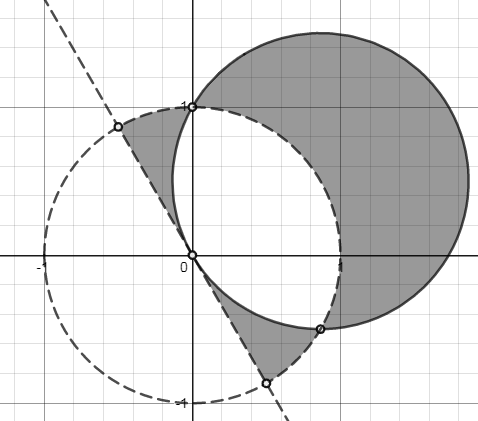
\includegraphics[width=0.8\linewidth]{../problems/Q_054/A_054.png}
\end{figure}
なお、境界線については、
\begin{itemize}
 \item 直線$y=-\sqrt{3}x$上の点は全て含めない。
 \item 円$x^2+y^2=1$上の点は全て含めない。
 \item 円$\disp \left(x-\frac{\sqrt{3}}{2}\right)^2+\left(y-\frac{1}{2}\right)^2=1$上の点は、上記2つにかからない範囲において含める。
\end{itemize}
